\documentclass[12pt,a4paper]{article}
\usepackage[utf8]{inputenc}
\usepackage[german]{babel}
\usepackage[T1]{fontenc}
\usepackage{amsmath}
\usepackage{amsfonts}
\usepackage{amssymb}
\usepackage{graphicx}
\usepackage[left=2.5cm,right=2.5cm,top=2cm,bottom=2cm]{geometry}
\usepackage{float}
\author{Gruppe C14 \\ Julián Häck, Martin Koytek, Lars Wenning, Erik Zimmermann}
\begin{document}
\section{Bestimmung der Erdbeschleunigung mit dem Pendel}
\subsection{Versuchsbeschreibung}
%Kurze Darstellung der physikalischen Grundlagen und Ziele der Versuche, %die zum Verständnis
%des Versuches/Protokolls benötigt werden. (max. 1 Seite)
Wir betrachten zunächst ein mathematisches Pendel ($J=m_Tl^2$), welches wir später durch die Verschiebung des Pendelkörpers ergänzen, um das physikalische Pendel betrachten zu können.
Die Bewegungsgleichung zum mathematischen Pendel nach der Kleinwinkelnäherung lautet:
\begin{equation}
J \cdot \ddot{\phi} = -m_s \cdot g \cdot l \cdot \phi 
\end{equation}
Mit $m_T=m_S$ und Lösen der Differential-Gleichung ergibt sich die allgemeine Lösung einer harmonischen Schwingung:
\begin{equation}
\phi(t)=A\cdot cos(\omega t) + B \cdot sin(\omega t)
\end{equation}
mit 
\begin{equation}
\omega=\sqrt{\frac{g}{l}}
\end{equation}
Wir bestimmen zunächst die Frequenz der Pendelstange ohne Gewicht. Dann bringen wir das Gewicht an und verschieben es auf der Stange bis die neue Frequenz mit der Alten übereinstimmt. Dadurch erreichen wir, dass wir das gesamte Pendel als homogenen Zylinder mit Radius $r_p$, der im Abstand $l_p$ um den Aufhängepunkt schwingt, annehmen können. 
\begin{equation}
J_p=\frac{1}{2}m_p r_p^2+m_p l_p^2
\end{equation}
Mit
\begin{equation}
\omega^2=\frac{D}{J}=\frac{m_p \cdot g \cdot l_p}{\frac{1}{2}m_p r_p^2+m_pl_p^2}
\end{equation}
ergibt sich:
\begin{equation}
g=\omega^2 l_p (1+\frac{r_p^2}{2 l_p^2}) 
\label{g}
\end{equation} 
\newpage
\subsection{Versuchsaufbau und Durchführung}
%Genaue Beschreibung der verwendeten Aufbauten unter Verwendung von Skizzen oder Photos
%Beschreibung der Messwerterfassungseinstellungen (eingestellte Messzeiten, Messbedingungen,
%Trigger, Anzahl der Messungen) und der Durchführung der Versuche. (max. 1 Seite)
\begin{figure}[H]
\centering
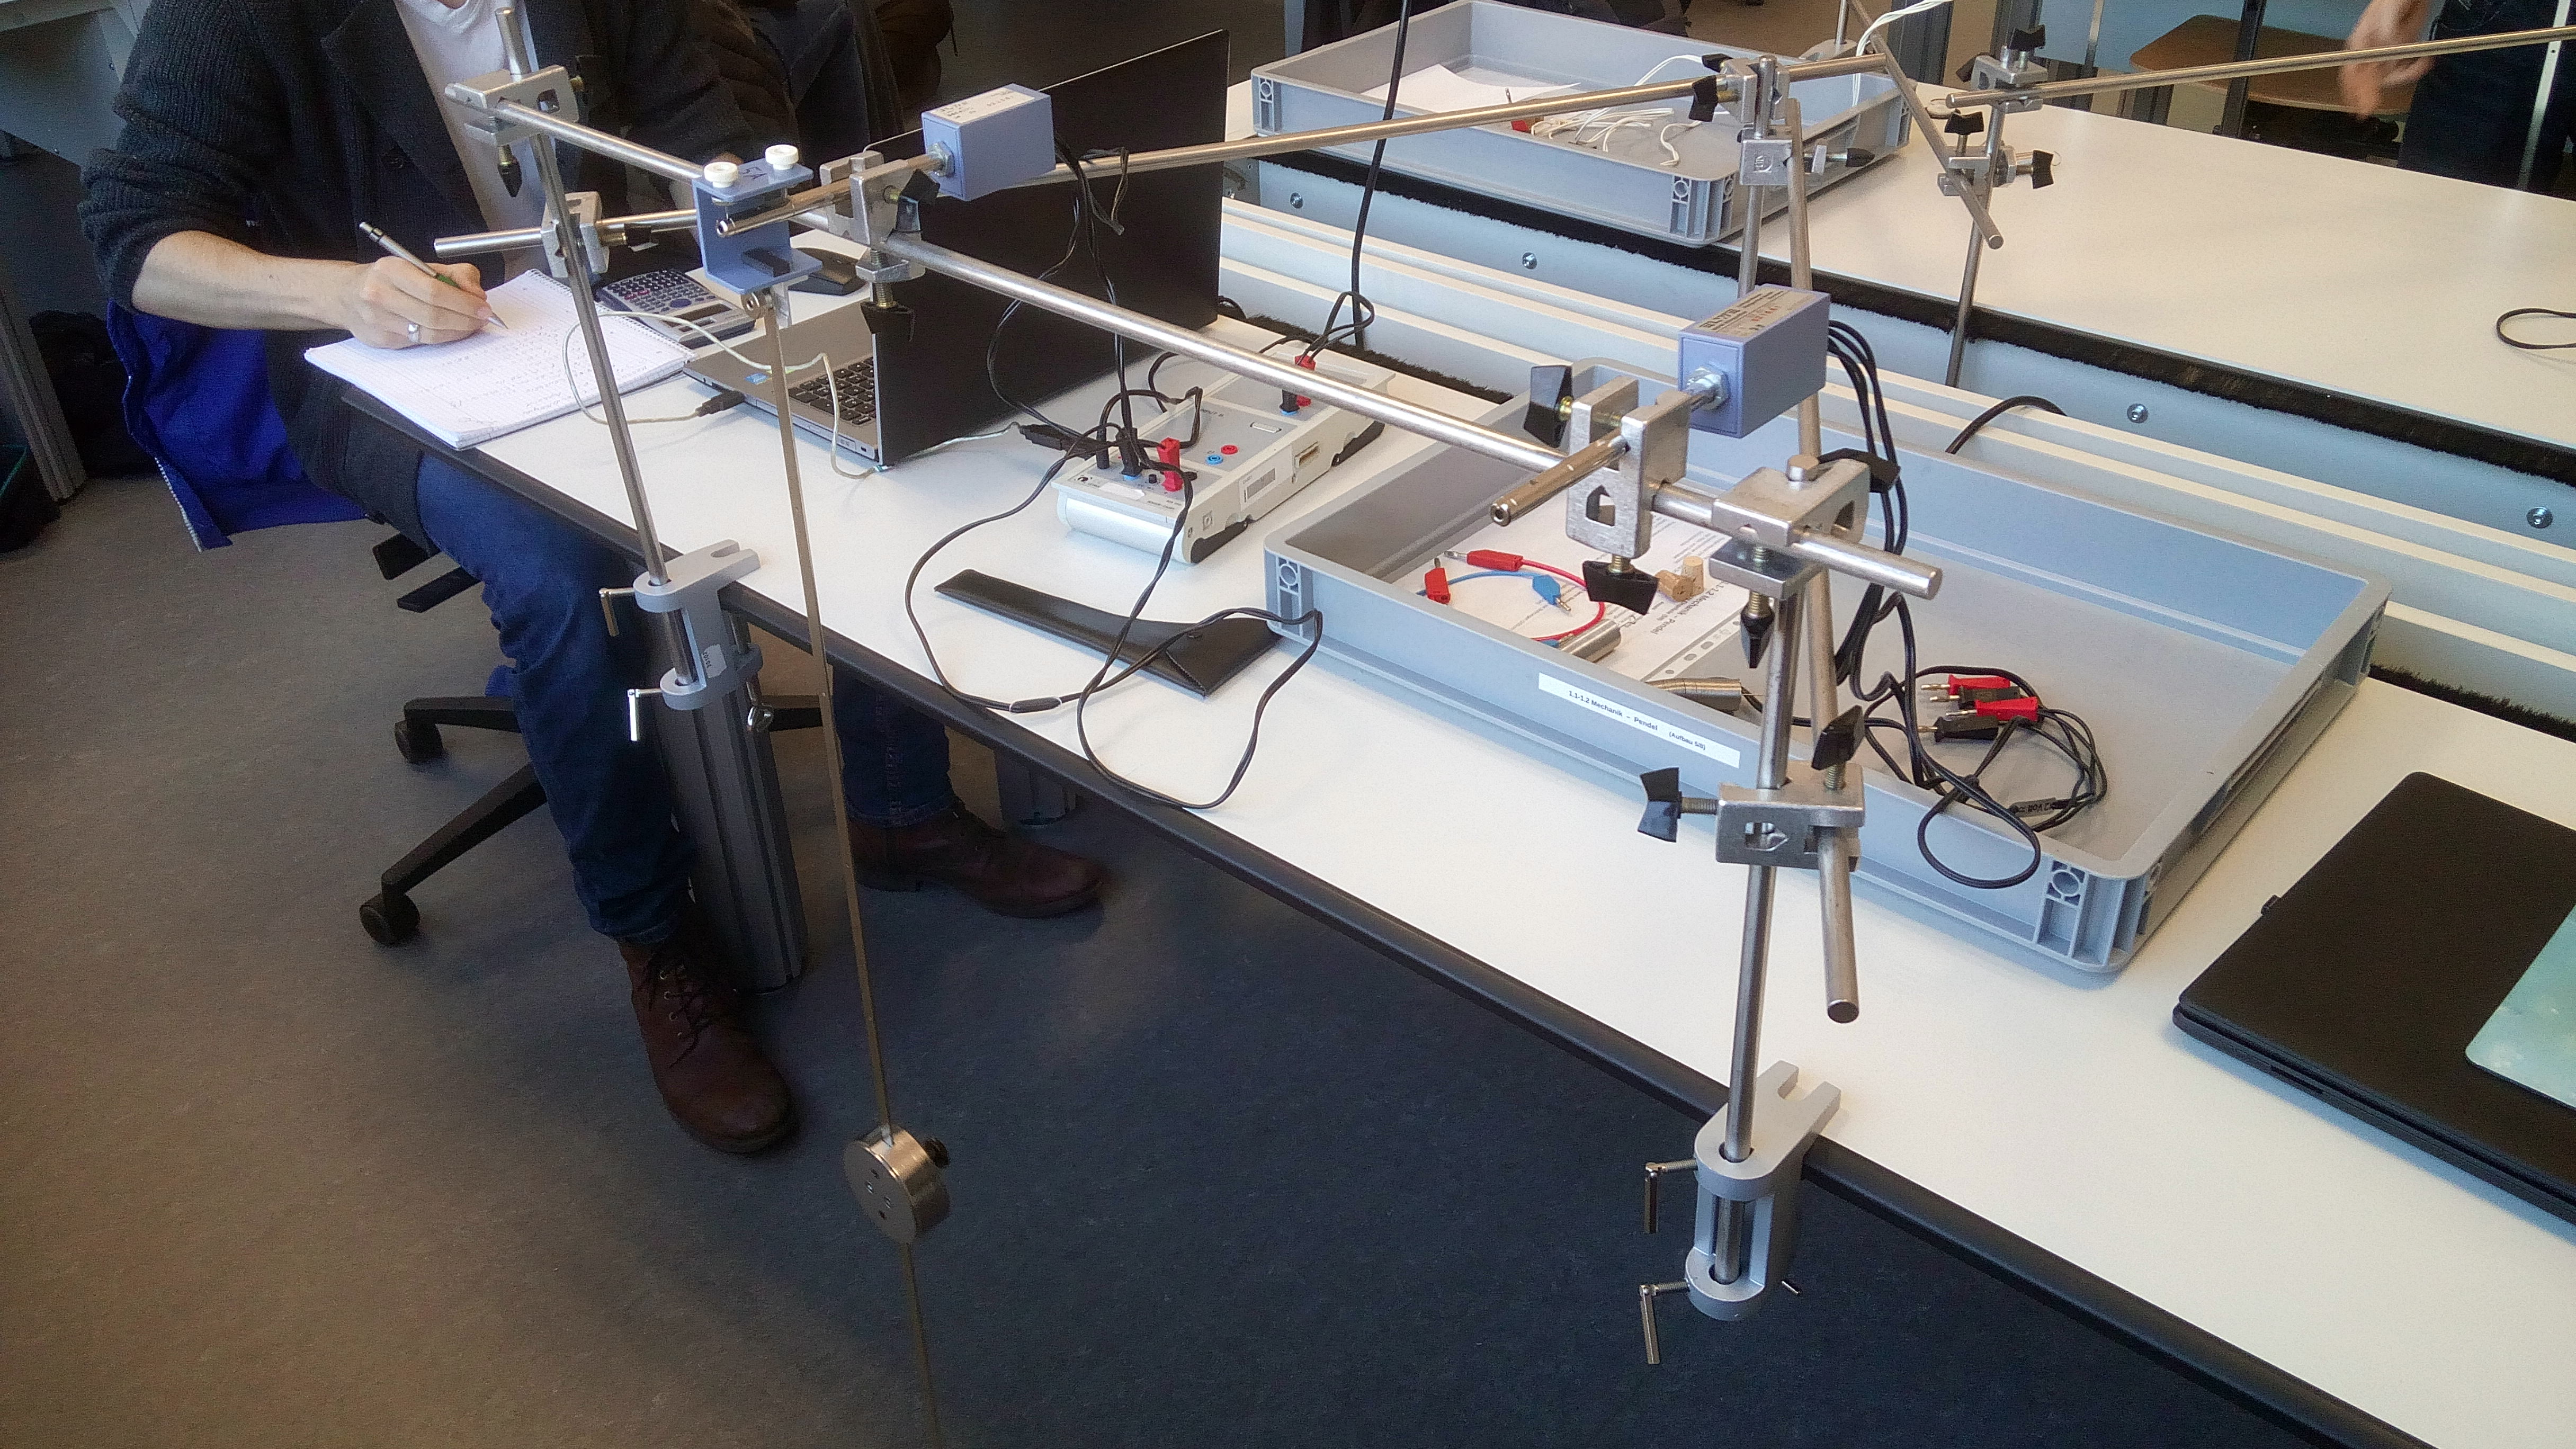
\includegraphics[scale=0.1]{Bilder/Einzelpendel.jpg}
\caption{Versuchsaufbau mit Pendelkörper}
\end{figure}
Unser Versuchsaufbau besteht aus einem Dreibein, um die Stabilität zu erhöhen, an dem dann der Winkelabnehmer befestigt wurde. \newline
In die Nut des Winkelabnehmers wurde dann die Aufhängung des Pendels aufgelegt.
Nun wurde zunächst die Pendelstange ohne Pendelkörper in Schwingung versetzt, die Hallspannung des Winkelabnehmers aufgezeichnet und die Frequenz per Fast-Fourier-Transformation (FFT) bestimmt. \newline
Anschließend wurde der Pendelkörper angebracht, das Pendel erneut ausgelenkt und die Schwingung aufgezeichnet. 
Dies wurde wiederholt bis die Frequenz mit der der Pendelstange ohne Pendelkörper übereinstimmte.
Dieser Aufbau wurde nun mehrmals in Schwingung versetzt und die Hallspannungen aufgezeichnet.
Zum Schluss wurde dann die Länge des Pendels, der Abstand des Pendelkörpers zum Aufhängepunkt und der Radius des Pendelkörpers gemessen.
\newline
Später haben wir bei der Auswertung alle Frequenzen neu über Ablesen der Nulldurchgänge bestimmt und damit aus Gleichung (\ref{g}) die Erdbeschleunigung bestimmt.
\subsubsection{Messwerterfassungseinstellungen}
\begin{center}
\begin{tabular}{c|c}
Messbereich & -1V..1V \\ 
\hline
Messintervall & 10ms \\ 
\hline
Messpunkte & 16000 \\ 
\hline
Messzeit & 160s \\ 
\end{tabular} 
\end{center}
\newpage
\subsubsection{Geräte}
Je Gruppe:
\begin{itemize}
\item 2 Hallsonden
\item 1 Laptop
\item 1 Sensor-Cassy
\item 1 Pendelstange mit Aufhängung
\item 1 Gewicht
\item Stativzubehör
\end{itemize}
\subsection{Versuchsauswertung}

\subsubsection{Rohdaten}
\begin{center}
\begin{tabular}{c|c|c}
 & Gruppe 1 & Gruppe 2 \\ 
\hline
Masse & 1.0207kg & 1.0217kg \\ 
$\sigma_{Masse}$ & 0.001kg & 0.001kg \\ 
Durchmesser des Gewichts & 0.08m & 0.084m \\ 
$\Rightarrow$ Radius & 0.04m & 0.042m \\ 
$\sigma_{Schieblehre}$ & 0.0005m & 0.0005m \\ 
$l_p$ & 0.6788m & 0.689m \\ 
$\sigma_{l_p}$ & 0.005m & 0.005m \\ 
Frequenz ohne Gewicht [FFT] & 0.6039Hz & 0.6030Hz \\ 
bsp. Frequenz mit Gewicht [FFT] & 0.6032Hz & 0.6011Hz \\ 
\end{tabular} 
\end{center}
$\sigma_{Masse}$: aus Angabe der Waage.\\
$\sigma_{Schieblehre}$: aus Angabe der Schieblehre. \\
$\sigma_{l_p}$: Durch Durchhängen und Verschieben des Maßbands, Mehrfachmessung der Einzellängen (Radius, Aufhängung, Stange selbst) abgeschätzt.\\
Abweichung Frequenz ohne Gewicht und mit Gewicht:
\begin{equation}
\Delta f=1-\frac{f_o}{f_m}
\end{equation}
\begin{figure}[H]\centering
\begin{tabular}{c|c|c}
 & Gruppe 1 & Gruppe 2 \\ 
\hline
$\Delta f$ & $-1.160\cdot 10^{-3}$ & $-3.161\cdot 10^{-3}$ \\ 
\end{tabular} 
\caption{Abweichungen der Frequenzen}
\label{Abweichungen der Frequenzen}
\end{figure}
\newpage
\subsubsection{Transformation der Rohdaten}
%Transformation der Rohdaten und Modellanpassung. (1 Seite)
Die Frequenzen der  Einzelmessungen mit Pendelkörper wurden folgendermaßen durch Ablesen bestimmt:
\begin{figure}[H]
\caption{Bestimmung von f}
\centering
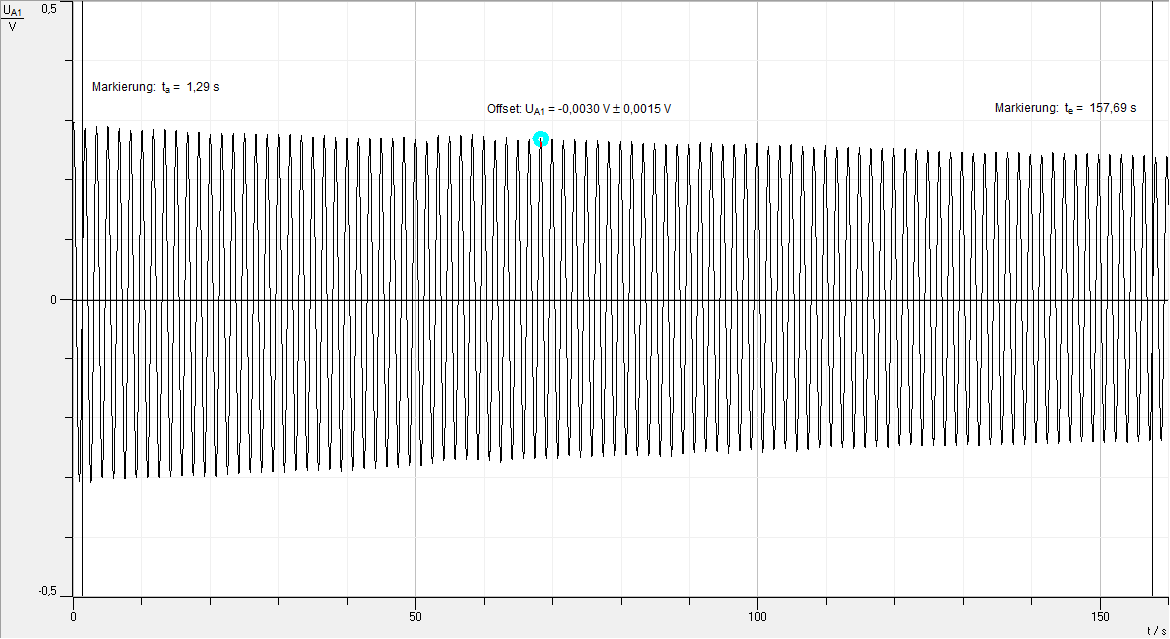
\includegraphics[scale=0.5]{Bilder/Erdbeschleunigung_bestimmungF.png}
\end{figure}
Hier:
\begin{equation}
t_a=1.29s, \hspace{1cm} t_e=157.69s.
\end{equation}
Die Fehler auf die Zeit ergeben sich aus der Auflösung zu:
\begin{equation}
\sigma_t=\frac{0.01}{\sqrt{12}}s
\end{equation}
Um die Nulldurchgänge ordentlich abzulesen, wurde der Mittelwert der Schwingung eingezeichnet. Hier: $U_{Offset} = -0,0030 V$.
Dann wurden die Perioden gezählt. Hier: $n=94$.
Mit Hilfe von:
%w=(2*np.pi*n)/(t_e-t_a)
%sig_w=2*np.pi*np.sqrt(2)*sig_t*n/((t_e-t_a)**2)
\begin{equation}
\omega=\frac{2\pi n}{t_e-t_a}
\end{equation}
und
\begin{equation}
\sigma_{\omega}=\frac{2\cdot \pi \sqrt{2}\cdot n \cdot \sigma_t}{(t_e-t_a)^2}
\end{equation}
wurden jeweils die Kreisfrequenz und deren Fehler bestimmt.
Aus diesen wurde dann durch:
\begin{equation}
g=\omega^2 l_p (1+\frac{r_p^2}{2 l_p^2}) 
\end{equation}
und
\begin{equation}
\sigma_g=\sqrt{(2\omega l_p (1+\frac{r_p^2}{2 l_p^2}))^2 \cdot \sigma_{\omega}^2+(\omega^2 \cdot \frac{r_p}{l_p})^2 \cdot \sigma_r^2+(\omega^2(1-\frac{r_p^2}{2 l_p^2}))^2 \cdot \sigma_l^2} 
\end{equation}
die Erdbeschleunigung und deren Fehler bestimmt.
Daraus ergaben sich folgende Ergebnisse:
\begin{figure}[H]\centering
\begin{tabular}{c|c|c|c|c}
Messung: & 1. & 2. & 3. & 4. \\ 
g: Gruppe 1 & 9.766 & 9.766 & 9.770 & / \\ 
$\sigma_g$: Gruppe 1 & 0.071 & 0.072 & 0.072 & / \\ 
g: Gruppe 2 & 9.838 & 9.839 & 9.842 & 9.845 \\ 
$\sigma_g$: Gruppe 2 & 0.071 & 0.071 & 0.071 & 0.071 \\ 
\end{tabular} 
\newline
\newline
Angaben in $\frac{m}{s^2}$
\end{figure}

Diese Ergebnisse wurden nun gewichtet gemittelt:
\begin{equation}
\bar{g} = \frac{\sum{\frac{g}{\sigma_g^2}}}{\sum{\frac{1}{\sigma_g^2}}}
\end{equation}
\begin{equation}
\sigma_{\bar{g}} = \sqrt{\frac{1}{\sum{\frac{1}{\sigma_g^2}}}}
\end{equation}
\begin{center}
\begin{tabular}{c|c|c}
 & Gruppe 1 & Gruppe 2 \\ 
\hline 
$\bar{g}$ & 9.767 & 9.841 \\ 
$\sigma_{\bar{g}}$ & 0.041 & 0.036 \\ 
\end{tabular} 
\newline
\newline
Angaben in $\frac{m}{s^2}$
\end{center}


\newpage
\subsubsection{Analyse und Fazit}
\begin{figure}[H]
\caption{Vergleich gewichteter Mittelwert gegen Einzelwerte und theoretischen Wert}
\centering
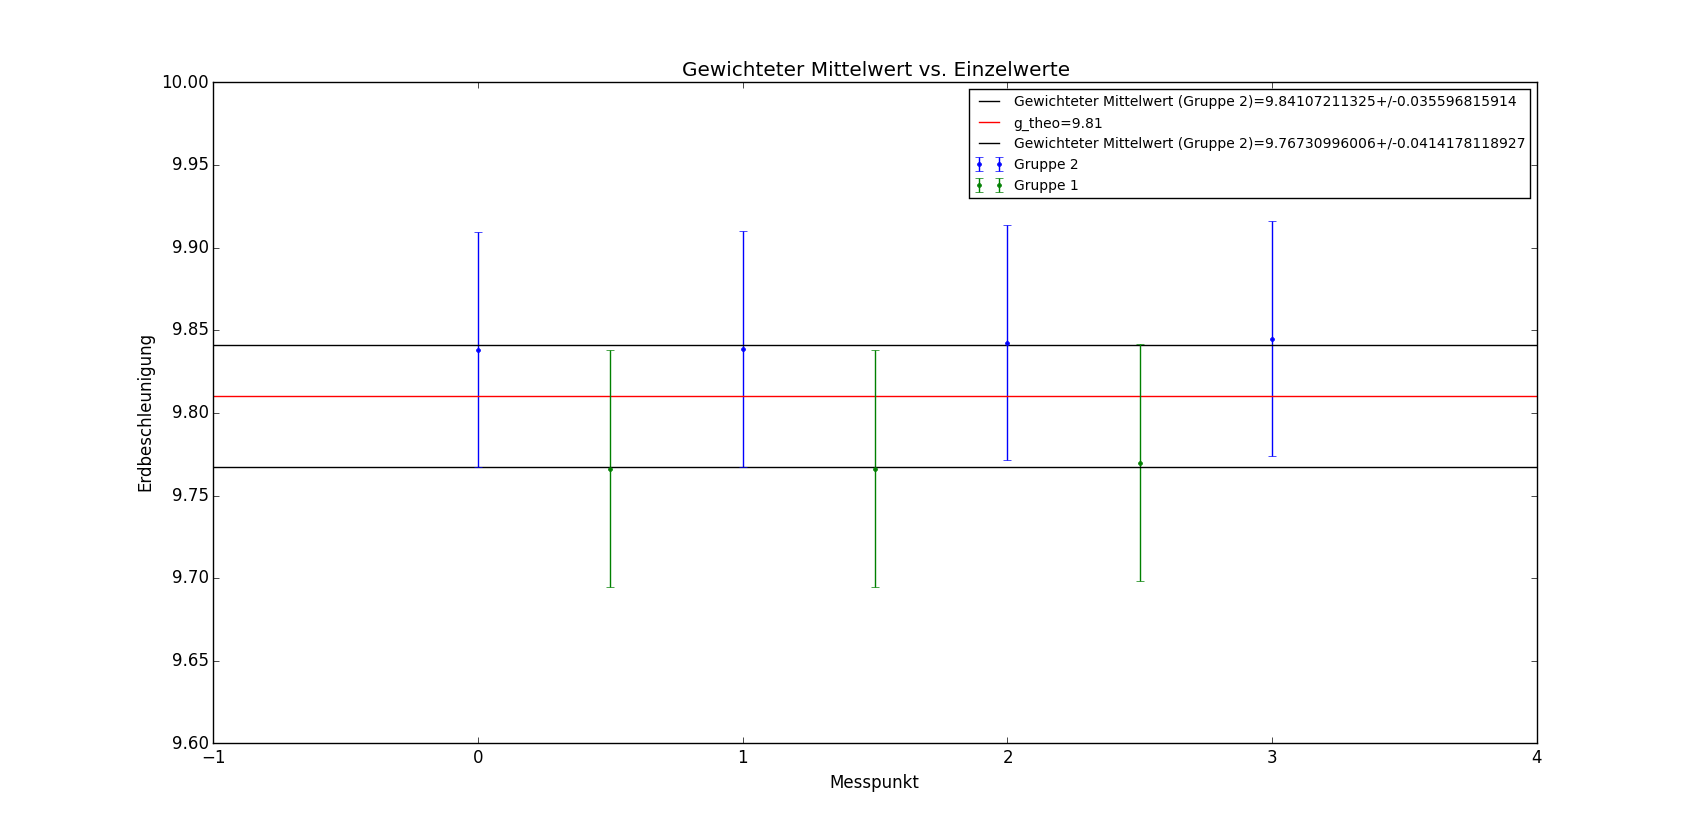
\includegraphics[scale=0.4]{Bilder/Erdbeschleunigung_alle_besserer_fehler.png}
\end{figure}
Auf dem Plot sehen wir in grün die Einzelwerte mit Einzelfehler für g der Gruppe 1 mit ihrem gewichteten Mittelwert, darüber ist in blau dasselbe für Gruppe 2 eingezeichnet. In rot sehen wir in der Mitte den theoretischen Wert von $g=9.81$.
\newline
Wie man sieht schneiden alle Fehlerbalken sowohl die gewichteten Mittelwerte, als auch den theoretischen Wert von g. Interessant hierbei ist, dass Gruppe 1 stets unterhalb des theoretischen Wertes geblieben ist und Gruppe 2 ausschließlich darüber.
Dies kann man durch die Annahme erklären, die wir weiter oben gemacht haben, nämlich, dass das Pendel mit Pendelkörper, wenn es die gleiche Frequenz wie das Pendel ohne Pendelkörper hat, durch einen Zylinder genähert werden kann. 
Wie in der Tabelle der Rohdaten zu sehen ist, sind die Frequenzen des Pendels mit und ohne Gewicht nicht exakt gleich (siehe Abbildung: \ref{Abweichungen der Frequenzen}). Dies wirkt sich auf unsere Näherung aus und erklärt so unsere Abweichung im obenstehenden Plot.\\

\textbf{Fazit}: \newline
Zusammenfassend kann man sagen, dass unsere Ergebnisse sehr zufriedenstellend sind. Sie weichen zwar systematisch vom theoretischen Wert ab, dies lässt sich aber durch die Näherung des homogenen Zylinders erklären.

\section{gekoppeltes Pendel}
\subsection{Versuchsbeschreibung}
%Kurze Darstellung der physikalischen Grundlagen und Ziele der Versuche, %die zum Verständnis
%des Versuches/Protokolls benötigt werden. (max. 1 Seite)
\begin{figure}[H]
\centering
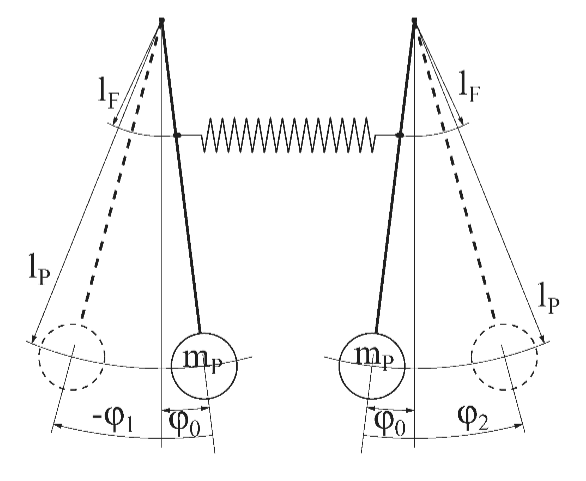
\includegraphics[scale=0.5]{Bilder/Gekoppeltes-Pendel.PNG}
\end{figure}

In diesem Versuch wird der Kopplungsgrad eines gekoppelten Pendels und die Federkonstante der Feder bestimmt, die für die Kopplung verantwortlich ist.
Die Feder erzeugt ein Drehmoment von
\begin{equation*}
M_{F,0}=-D_F \cdot x_0 \cdot l_F
\end{equation*}
welches durch das von der Schwerkraft erzeugte Drehmoment 
\begin{equation*}
M_{S,0}=m \cdot g \cdot l_s \cdot \phi_0
\end{equation*}
kompensiert wird.
So ergibt sich für das gesamte Drehmoment, wenn ein Pendel um $\phi_2$ ausgelenkt wird:
\begin{equation*}
M_2=-m \cdot g \cdot l_s \cdot \phi_2 - D_F \cdot l_F^2 \cdot \phi_2
\end{equation*}
Daraus ergibt sich für die Bewegungsgleichungen der beiden Pendel:
\begin{align*}
\ddot{\phi_1}=-\omega_s^2 \cdot \phi_1 + \Omega^2 \cdot (\phi_2 - \phi_1) \\
\ddot{\phi_2}=-\omega_s^2 \cdot \phi_2 - \Omega^2 \cdot (\phi_2 - \phi_1)
\end{align*}
Dabei sind:
\begin{align*}
\omega_s~und~\omega_{sf}=\sqrt{\omega_s^2+2\Omega^2}
\end{align*}
Lösungen dieses Systems aus gekoppelten Differenzialgleichungen.
Der Kopplungsgrad wird definiert als:
\begin{align}
\kappa =\frac{D_F l_F^2}{mgl_s + D_F l_F^2}= \frac{\omega_{sf}^2-\omega_{s}^2}{\omega_{sf}^2+\omega_s^2}
\end{align}
Um die Federkonstante zu bestimmen, wird $\frac{1}{\kappa}$ gegen $\frac{1}{l_F^2}$ aufgetragen:
\begin{align}
\frac{1}{\kappa}=1+\frac{ml_sg}{D_F}\cdot \frac{1}{l_F^2}
\label{k}
\end{align}
Zur Überprüfung wird die Federkonstante auch durch das Hook'sche Gesetz:
\begin{align}
m \cdot g = -D_F \cdot x
\label{Hook}
\end{align}
bestimmt.
\subsection{Versuchsaufbau und Durchführung}
%Genaue Beschreibung der verwendeten Aufbauten unter Verwendung von Skizzen oder Photos
%Beschreibung der Messwerterfassungseinstellungen (eingestellte Messzeiten, Messbedingungen,
%Trigger, Anzahl der Messungen) und der Durchführung der Versuche. (max. 1 Seite)
\begin{figure}[H]
\centering
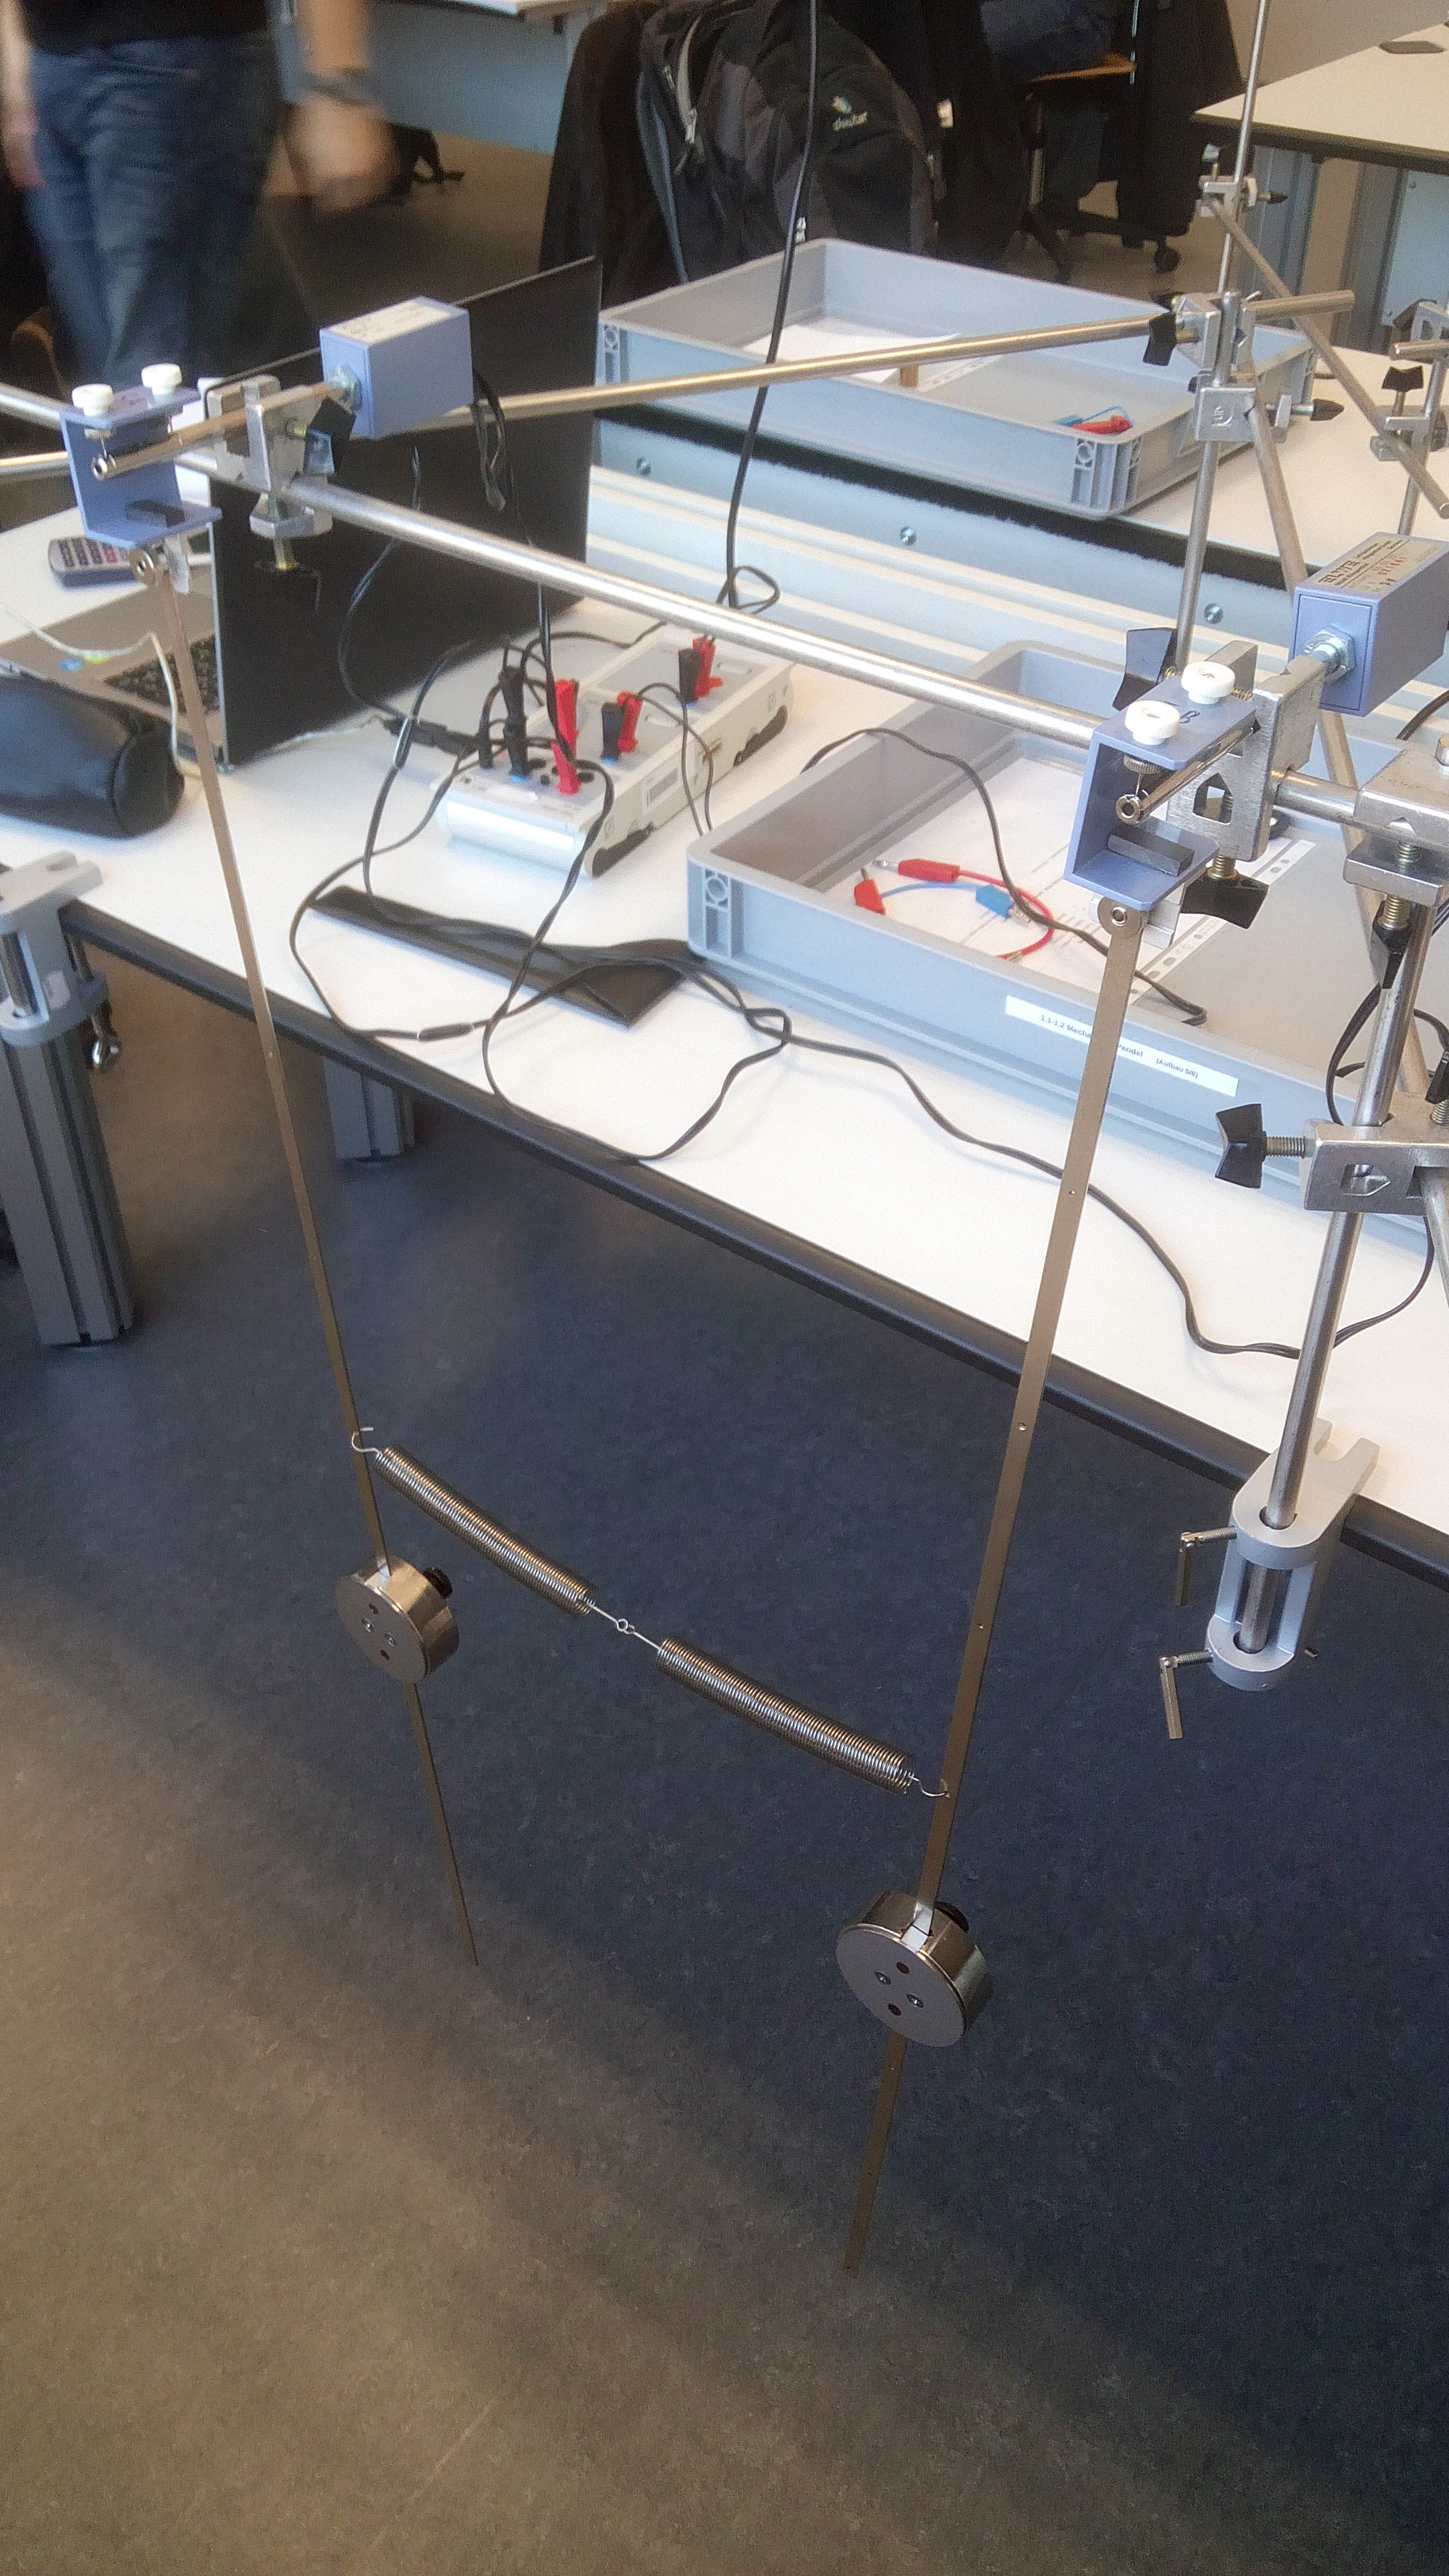
\includegraphics[scale=0.1]{Bilder/Doppelpendel.jpg}
\caption{gekoppeltes Pendel}
\end{figure}
Der Versuchsaufbau des gekoppelten Pendel ist der gleiche wie beim Einzelpendel nur, dass ein zusätzliches, möglichst identisches Pendel verwendet wird. Dieses Pendel wird auf gleicher Höhe im Abstand von ca. 50cm befestigt und mit einer Feder an das andere Pendel gekoppelt. Die Befestigungshöhe der Feder wird dabei variiert, um die Kopplung zu verändern (siehe: \ref{k}). Mittels Linearer Regression lässt sich dann ein Wert für die Federkonstante D bestimmen. \newline
Des Weiteren wurde die Federkonstante aus dem Hook'schen Gesetz (siehe: \ref{Hook}) bestimmt. Dazu haben wir mit verschiedenen Gewichten die Feder belastet und die Auslenkung gegenüber der Ruhelage gemessen.
Zuletzt wurden noch die Pendelkörper gewogen.
\subsection{Versuchsauswertung}
\subsubsection{Rohdaten}
\begin{figure}[H]
\centering
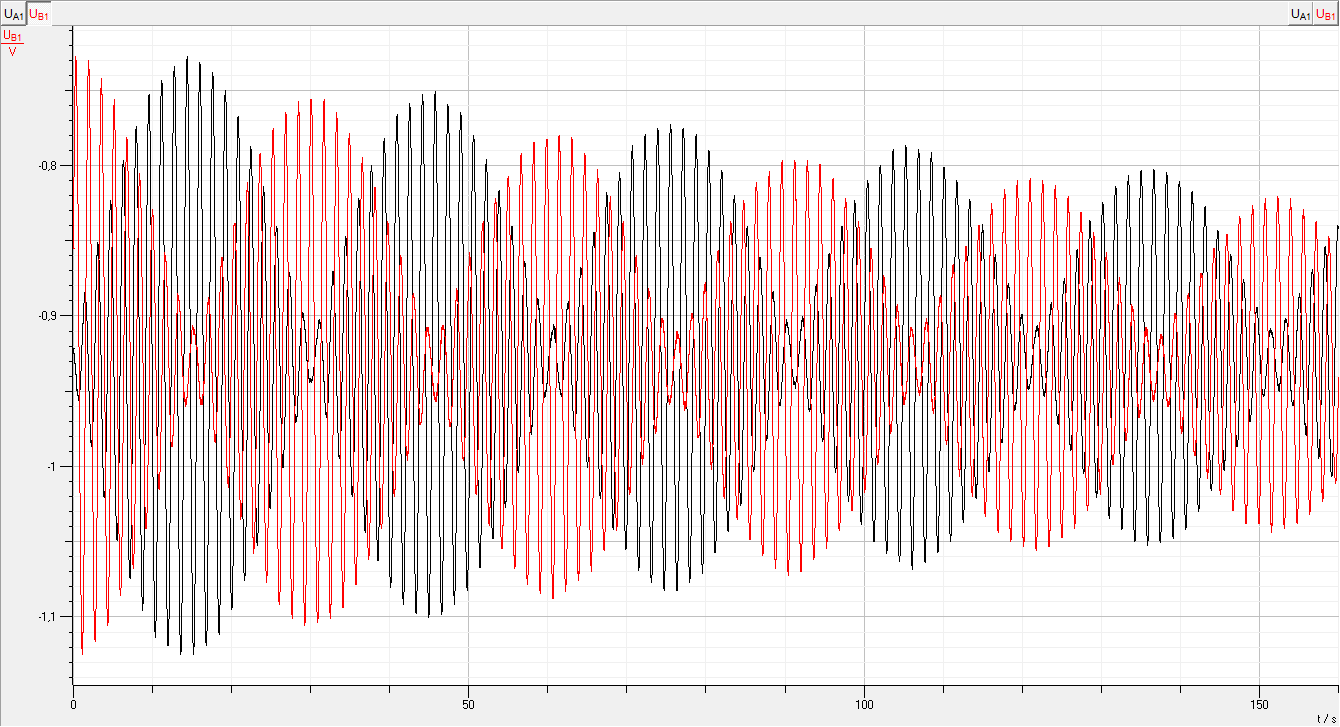
\includegraphics[scale=0.6]{Bilder/Schwebung.png}
\caption{Schwebung Loch 2}
\end{figure}
\begin{figure}[H]
\centering
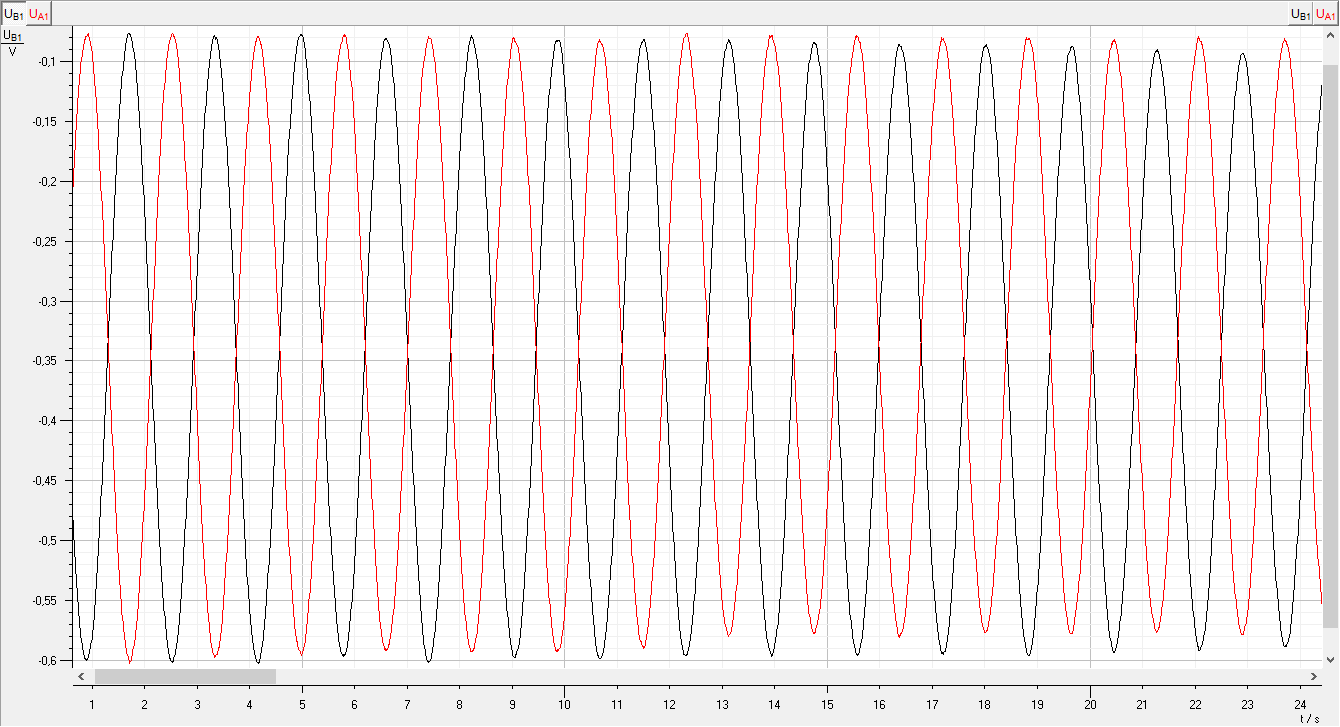
\includegraphics[scale=0.6]{Bilder/Gegensinnig.png}
\caption{Gegensinnige Auslenkung}
\end{figure}
\begin{figure}[H]
\centering
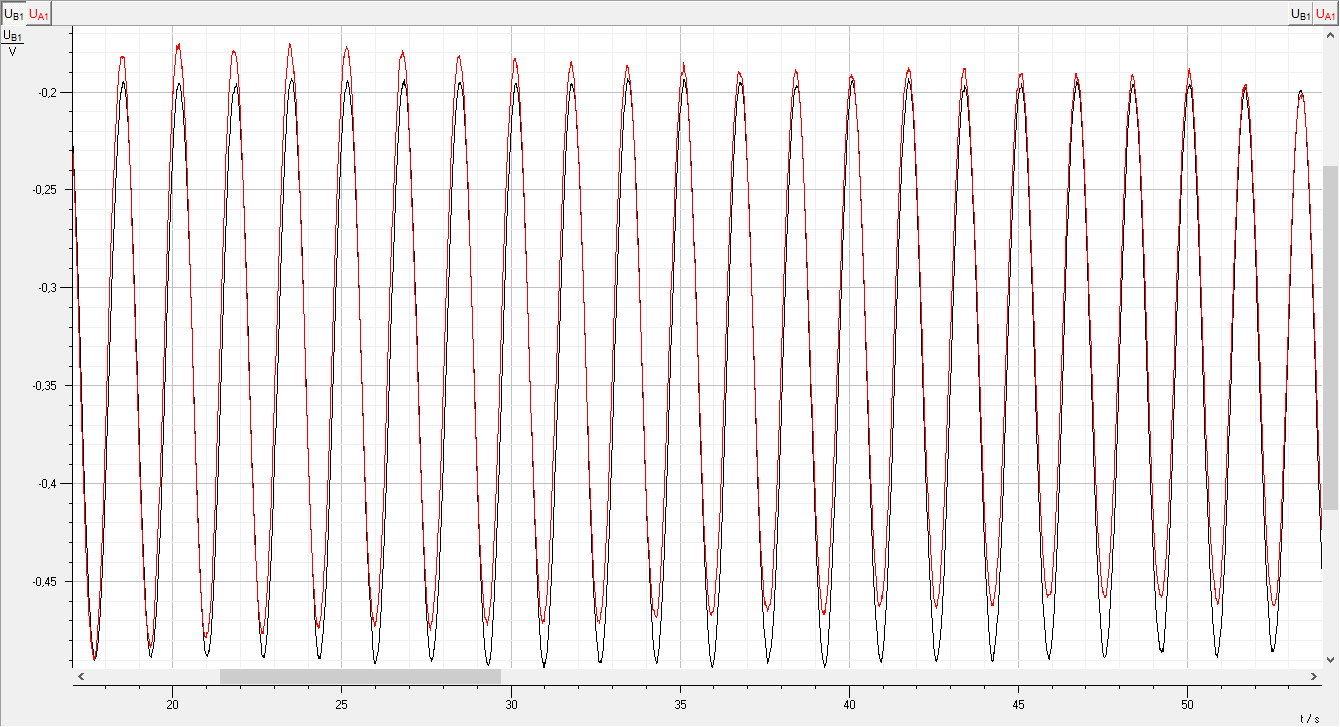
\includegraphics[scale=0.5]{Bilder/Gleichsinnig.png}
\caption{Gleichsinnige Auslenkung}
\end{figure}
\textbf{Daten zur Berechnung von D aus Gleichung (\ref{Hook}):}\newline
Die Ablesefehler wurden bei den Längenmessungen zu $\sigma_x=0.1cm$ bestimmt.\newline
Auslenkung: $x=x_{gemessen}-x_0$ \newline
Ruhelage der Feder Gruppe 1: $x_0=21.6cm$
\begin{table}[H]\centering
\caption{Daten Hook Gruppe 1}
\begin{tabular}{c|c|c|c}
Auslenkung in cm & Fehler in cm & angehängte Masse in g & Fehler der Waage in g\\ 
\hline
$x_1=11.3$& $\sigma_{x_1}=0.1$& $m_1=60$& $\sigma_{m_1}=0.1$\\ 
$x_2=18.7$& $\sigma_{x_2}=0.1$& $m_2=100$& $\sigma_{m_2}=0.1$\\
$x_3=14.9$& $\sigma_{x_3}=0.1$& $m_3=80$& $\sigma_{m_3}=0.1$\\
\end{tabular} 
\end{table}
Ruhelage der Feder Gruppe 2: $x_0=22.8cm$
\begin{table}[H]\centering
\caption{Daten Hook Gruppe 2}
\begin{tabular}{c|c|c|c}
Auslenkung in cm & Fehler in cm & angehängte Masse in g & Fehler der Waage in g\\ 
\hline
$x_1=22.2$& $\sigma_{x_1}=0.1$& $m_1=120.5$& $\sigma_{m_1}=0.1$\\ 
$x_2=18.3$& $\sigma_{x_2}=0.1$& $m_2=103$& $\sigma_{m_2}=0.1$\\
$x_3=8.9$& $\sigma_{x_3}=0.1$& $m_3=50.3$& $\sigma_{m_3}=0.1$\\
$x_4=3.3$& $\sigma_{x_4}=0.1$& $m_4=20$& $\sigma_{m_4}=0.1$\\
\end{tabular} 
\end{table}
\begin{table}[H]\centering
\caption{Löcher mit ihren Abständen vom Aufhängepunkt}
\begin{tabular}{c|c|c|c}
Löcher &Gruppe 1&Gruppe 2\\ 
\hline
$1.$& $15.8cm$& $16.4cm$\\ 
$2.$& $27.8cm$& $28.5cm$\\
$3.$& $40.4cm$& $41cm$\\
$4.$& $52.9cm$& $53.5cm$\\
$6.$& $77.6cm$& $78.5cm$\\ 
$7.$& $89.6cm$& $90.5cm$\\
$8.$& $101.6cm$& $102.6cm$\\
\end{tabular} 
\end{table}
\newpage
\subsubsection{Transformation der Rohdaten/Analyse}
Aus der Schwebung des Doppelpendels ergeben sich mit Fast-Fourier-Transformation $\omega_s$ und $\omega_{sf}$ durch $\omega=2\pi f$:
\begin{figure}[H]
\centering
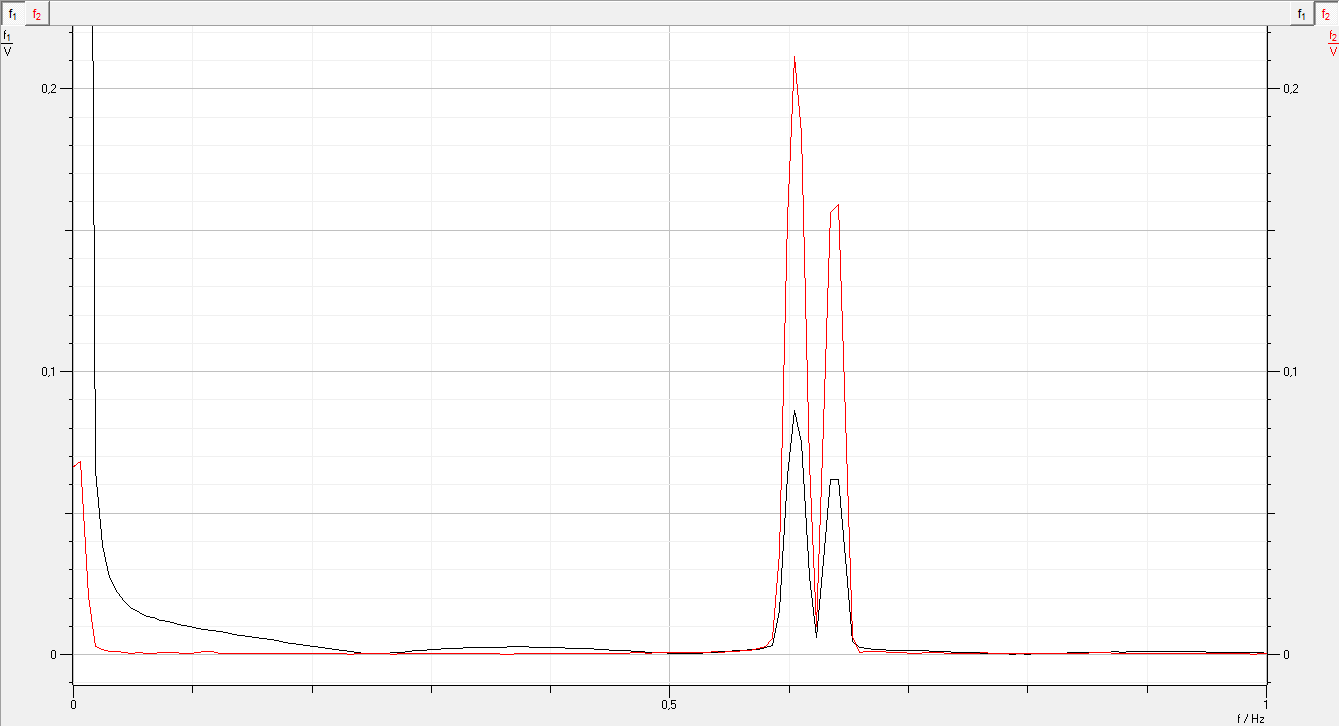
\includegraphics[scale=0.6]{Bilder/FFT-Schwebung.png}
\caption{FFT-Schwebung}
\end{figure}
$~$ \newline
Die geringere Frequenz $f_s$ sieht man bei der gleichsinnigen und die größere Frequenz $f_{sf}$ bei der gegensinningen Auslenkung.
\newline
Für die verschiedenen Positionen der Feder wurde das 5. Loch vom Pendelkörper blockiert und die Kopplung des ersten Lochs war so gering, dass wir nur eine Frequenz ermitteln konnten, so dass wir diese Werte im Folgenden nicht mehr betrachten.
Für die anderen Positionen wurde jeweils per FFT die Frequenzen mit ihren Ablesefehlern bestimmt. Der Ablesefehler wurde durch mehrfache Peakschwerpunktbestimmung ermittelt.
\begin{figure}[H]
\centering
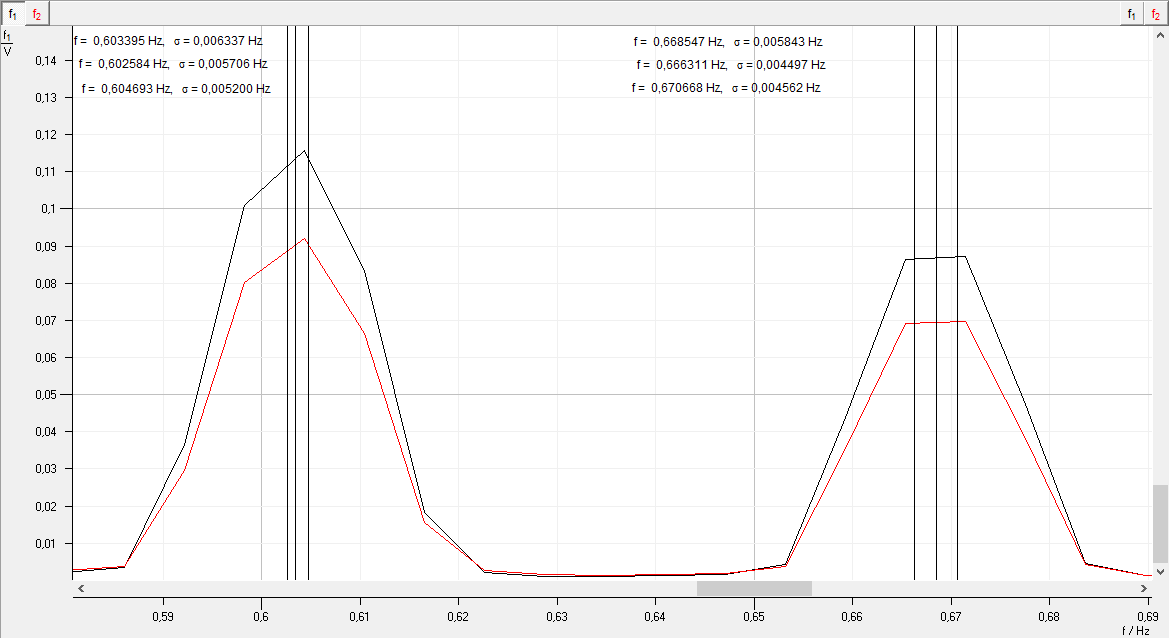
\includegraphics[scale=0.42]{Bilder/fft_Fehlermessung.png}
\caption{Peakschwerpunktsbestimmung}
\end{figure}

\begin{figure}[H]
\centering
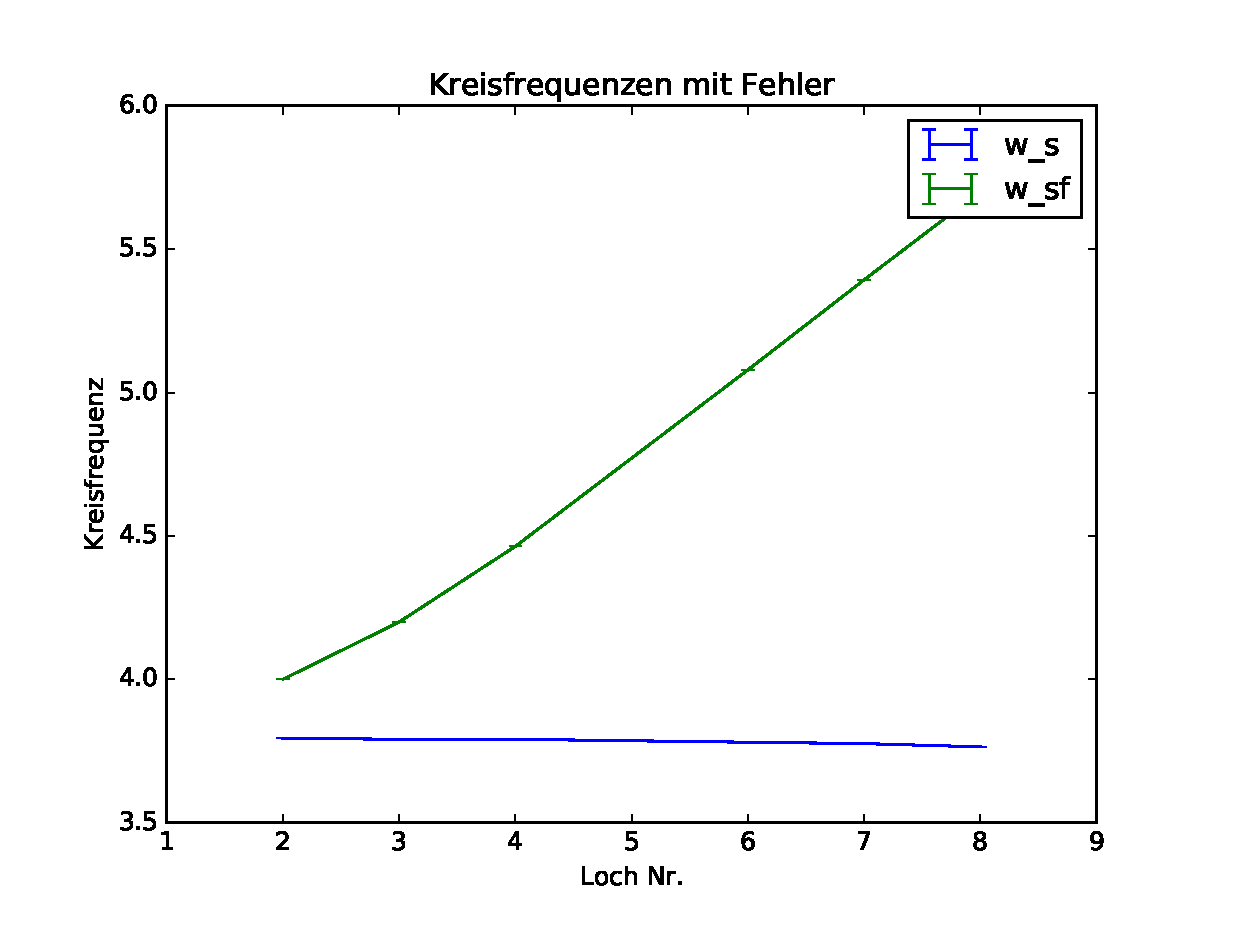
\includegraphics[scale=0.7]{Bilder/Kreisfrequenzen_fuer_Kappa.eps}
\caption{Loch/Frequenzen}
\end{figure}
Aus diesen Frequenzen wurde anschließend $\kappa$ durch Gleichung (\ref{k}) bestimmt.
\newline
Nun wurde $\frac{1}{\kappa}$ gegen $\frac{1}{l_F^2}$ aufgetragen, um aus der Steigung die Federkonstante bestimmen zu können.
\begin{figure}[H]
\centering
\caption{}
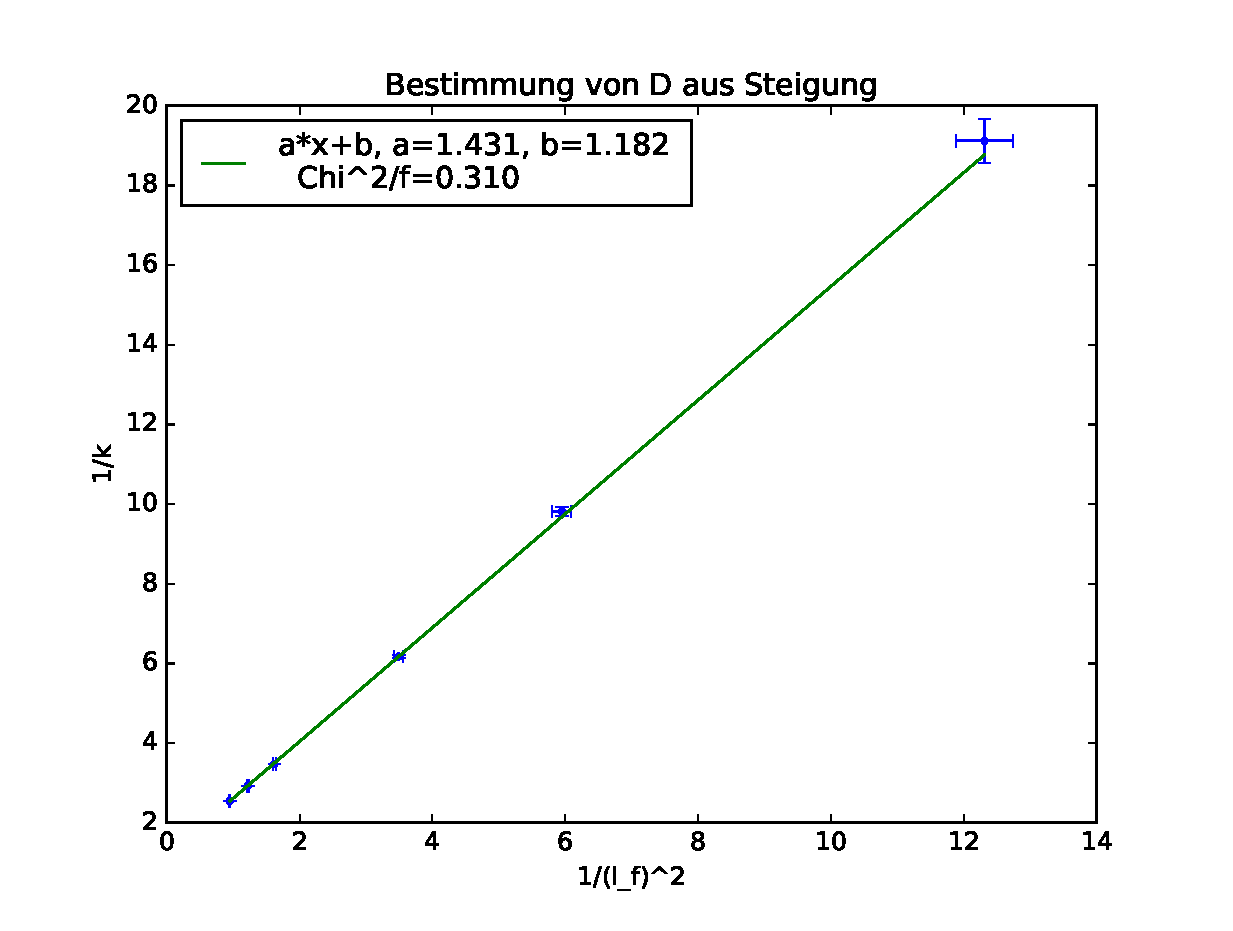
\includegraphics[scale=0.7]{Bilder/Bestimmung_D_linreg.eps}
\end{figure}
Die gesuchte Federkonstante D ergibt sich dann aus:
\begin{align}
D_F=m \cdot l_s \cdot \frac{g}{a}\\
\sigma_{D_F}=m \cdot \sqrt{(g\cdot \frac{\sigma_{l_s}}{a})^2+(g\cdot l_s \cdot \frac{\sigma_a}{a^2})^2+(l_s \cdot \frac{\sigma_g}{a})^2}
\end{align}
Wobei hier g mit entsprechenden Fehlern aus dem Einzelpendelversuch benutzt wurde.
\begin{table}[H]\centering
\caption{$D_F$ aus Doppelpendel}
\begin{tabular}{c|c}
Gruppe 1 & Gruppe 2\\ 
\hline
$D_F=4.9636\frac{1}{m}$& $D_F=4.8491 \frac{1}{m}$\\ 
$\sigma_{D_F}=0.1622 \frac{1}{m}$& $\sigma_{D_F}=0.0609 \frac{1}{m}$\\
\end{tabular} 
\end{table}
\begin{figure}[H]
\caption{}
\centering
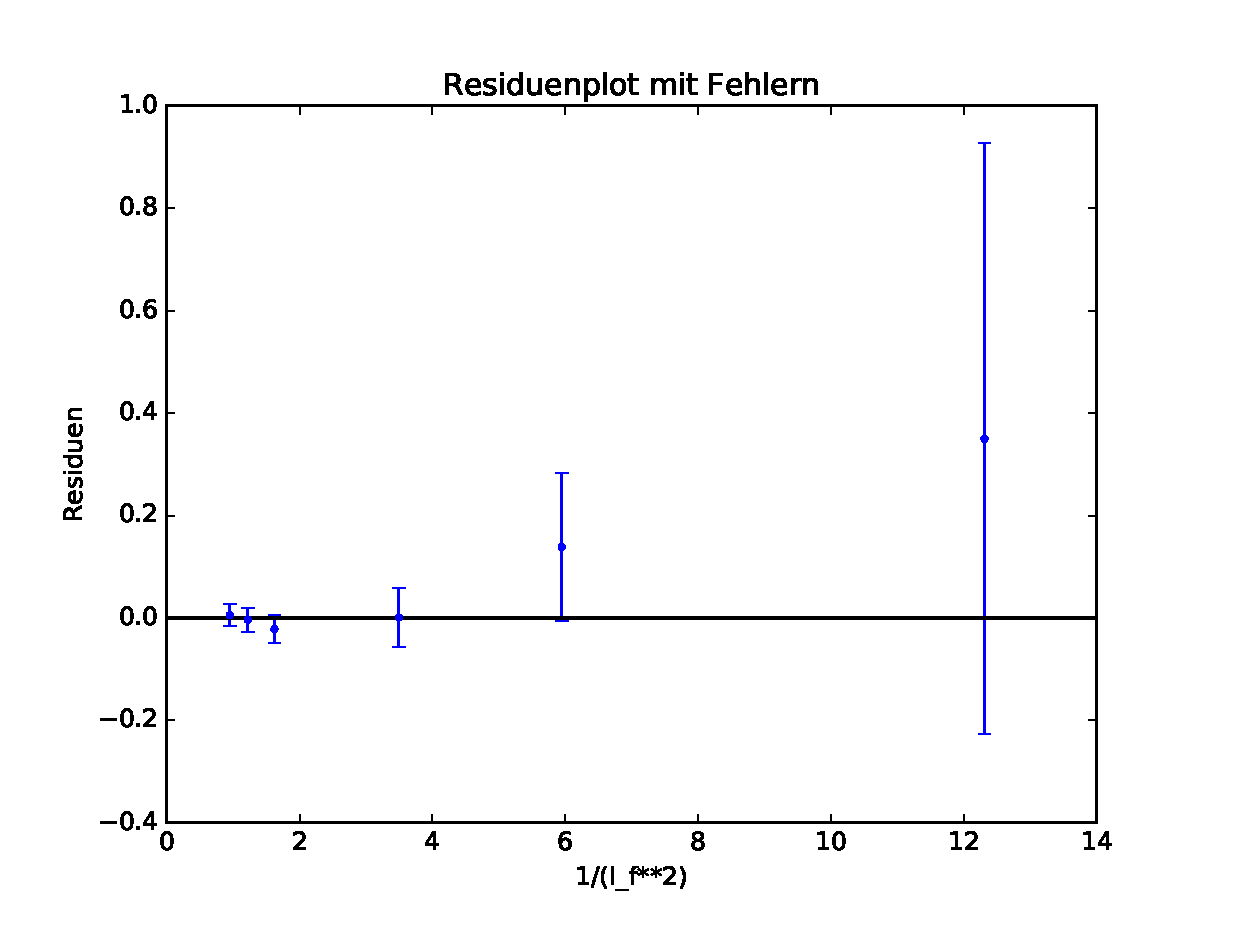
\includegraphics[scale=0.8]{Bilder/Bestimmung_D_Residuen.eps}
\end{figure}

Nun wurde zum Vergleich die Federkonstante noch einmal über das Hook'sche Gesetz (siehe: \ref{Hook}) bestimmt: 
\begin{figure}[H]
\caption{}
\centering
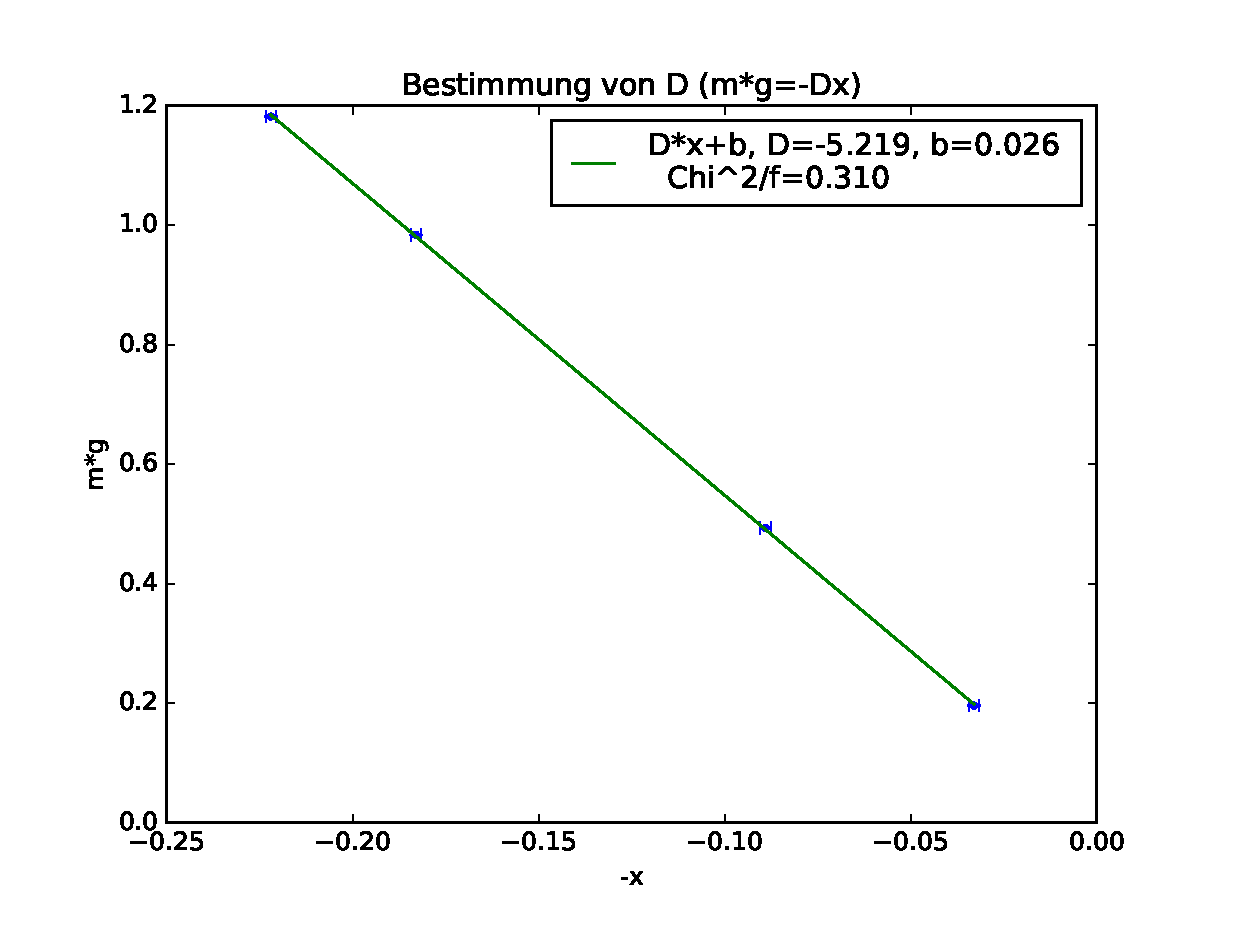
\includegraphics[scale=0.8]{Bilder/Hook_linreg.eps}
\end{figure}
\begin{equation*}
D_F=-\frac{m\cdot g}{x_0}
\end{equation*}
\begin{table}[H]\centering
\caption{$D_F$ aus Hook}
\begin{tabular}{c|c}
Gruppe 1 & Gruppe 2\\ 
\hline
$D_F=5.2671 \frac{1}{m}$& $D_F=5.219 \frac{1}{m}$\\ 
$\sigma_{D_F}=0.102 \frac{1}{m}$& $\sigma_{D_F}=0.0246 \frac{1}{m}$\\
\end{tabular} 
\end{table}
\begin{figure}[H]
\caption{}
\centering
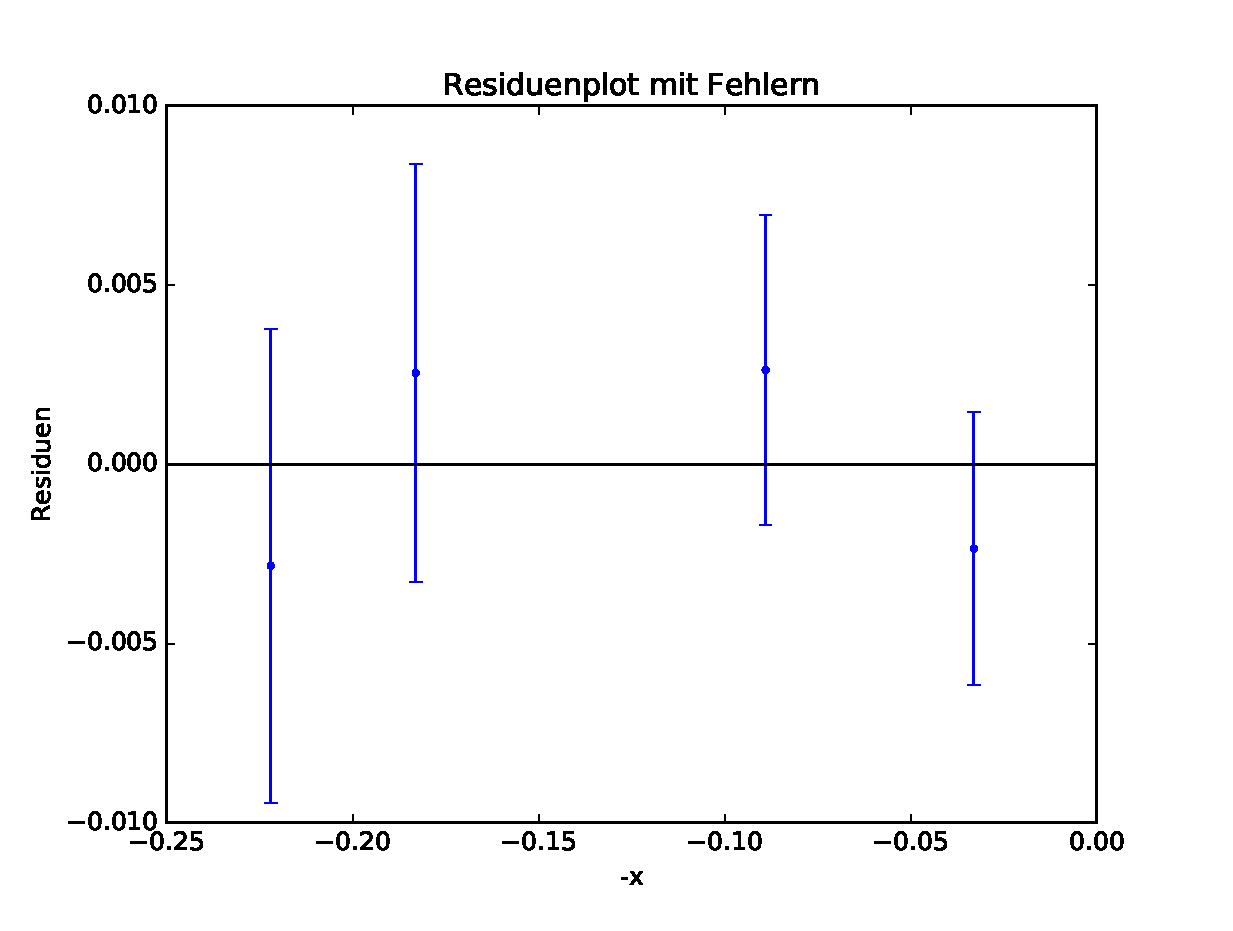
\includegraphics[scale=0.8]{Bilder/Hook_residuen.eps}
\end{figure}

\subsubsection{Fazit}
%Diskussion der Ergebnisse und Vergleich der erzielten Ergebnisse mit theoretischen Vorhersagen.
%(1 Seite)
Unsere Ergebnisse bei der Berechnung der Federkonstante stimmen mit ihren Fehlern nicht ganz überein. Bei Gruppe 2 gibt es sogar deutliche Abweichungen. Nach langer Diskussion erklären wir uns dies durch die Näherung unseres Pendels an einen homogenen zylindrischen Pendelkörper mit masseloser Pendelstange, die durch die angepasste Frequenz an die Pendelstange ohne Pendelkörper gegeben wird. Gruppe 2 hat hier eine Anpassung mit einem drei mal größeren Fehler auf die Frequenz (siehe: \ref{Abweichungen der Frequenzen}). Diese Ungenauigkeit in der Näherung zieht sich als systematischer Fehler durch die gesamte Rechnung. Dass wir nur statistische Fehler betrachtet haben, die Systematik aber einen nicht geringen Anteil am Fehler hat, erklärt unsere Abweichung der Ergebnisse aus dem Doppelpendel und der Hook'schen Federmessung.
\newline
Bei den Linearen Regressionen kann man erkennen, dass die Geraden alle Fehlerkästen schneiden.
Auch die Residuenplots entsprechen unseren Erwartungen, es sind keine Systematiken erkennbar. Somit sind unsere statistischen Fehler im Rahmen unserer Erwartungen.
\end{document}